
\section{Objectives}
By the end of this laboratory experiment, students are expected to learn how to:

\begin{itemize}

\item utilize basic logic gates to implement combinational logic circuits, and 
  
\item design and implement a simple digital system to indicate the safe operation of a sealed liquid tank.
   
\end{itemize}

\section{Parts}
\label{sec:partsEx13}
The following parts are required to conduct this laboratory experiment. %
%
\begin{enumerate}           
\item Breadboard
\item Agilent 33210A waveform generator
\item Agilent E3630A power supply
\item One SN7404\footnote{See datasheet at \url{http://www.ti.com/lit/ds/symlink/sn54ls04-sp.pdf}} NOT Gate IC
\item Two SN7408\footnote{See datasheet at \url{http://www.ti.com/lit/ds/symlink/sn74ls08.pdf}}   AND Gate ICs
\item One SN7432N\footnote{See datasheet at \url{http://www.ti.com/lit/ds/symlink/sn54ls32.pdf}}  OR Gate IC
\item Three LEDs (green, yellow, and red) 
  
\item Six $1~[\kilo\ohm]$ resistors 
\end{enumerate}


\section{Introduction}
\label{sec:introduction}

This laboratory exercise is meant to introduce concepts of digital circuits through designing a simple digital system that implements the safe operation of a sealed liquid tank in a chemical factory. The design and implementation of such a digital system is very similar to examples of combinational logic circuits provided in~\cite[Ch.~3]{Dueck2005-Digital}. Figure~\ref{fig:liquidTank}  shows a sealed liquid tank where three sensors, the level sensor (L), temperature sensor (T), and the pressure sensor (P) are installed to monitor the liquid level, the temperature, and the pressure of the tank, respectively. The tank is preset with threshold values of the liquid level, the temperature, and the pressure. If any of these quantities (\textit{i.e.,}~liquid level, temperature, or pressure) is above (below) the threshold value, the corresponding sensor generates a logic HIGH (LOW) signal. %The logic HIGH (LOW) signal is  denoted with binary number $1(0).$    


\begin{figure}[h]
    \centering
    \includegraphics{figs/ipe/lab_10/liquidTank.eps}
    \caption{A sealed liquid tank equipped with sensors.}
    \label{fig:liquidTank}
\end{figure}


The three sensors monitor the operation of the tank. The safety system to be designed has three LEDs: green, yellow, and red, where the cathode terminals of the LEDs are connected in series with $1~[\kilo\ohm]$ resistors.  The green LED indicates the tank is safe. The yellow LED illuminates to give a warning signal when one or more sensors generate logic HIGH signals indicating the corresponding quantities (liquid level, temperature, or pressure)  exceeded their threshold levels. If all of the sensors generate logic HIGH signals, the red LED illuminates indicating  a  danger condition within the tank.

\subsection{Safety System with Active-High Logic}
\label{sec:safetySystemAH}
The status of the tank will be represented by output LEDs that will use active-high logic (\textit{i.e.,}~logic HIGH is represented with binary value $1$ and logic LOW is represented with binary value $0$). The block diagram of the chemical tank safety system to be designed in this laboratory exercise is given in Figure~\ref{fig:safetySysNoClock}.
%
\begin{figure}[h]
    \centering
    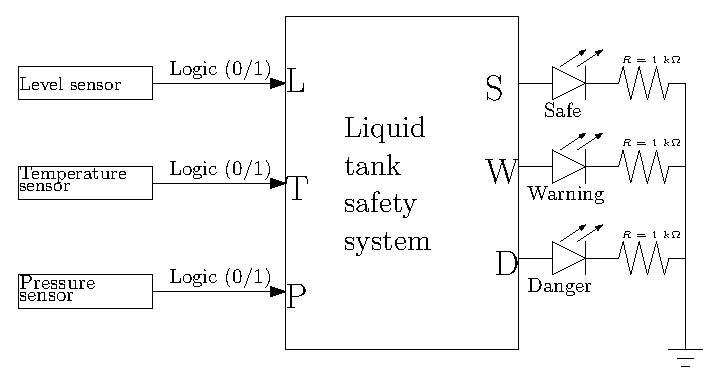
\includegraphics{figs/ipe/lab_10/safetySysNoClock.eps}
    \caption{Block diagram of the liquid tank safety system using active-high logic.}
    \label{fig:safetySysNoClock}
\end{figure}
%
The three inputs to the safety system are denoted with $L,$ $T,$ and $P$ which are connected to the level, temperature, and the pressure sensors, respectively. If an input is a logic $1 (0),$ the corresponding sensor generates a logic HIGH (LOW) signal. There are three outputs for the safety system: Safe (S), Warning (W), and Danger (D). The output signals S, W, and D are connected to the green, yellow, and red LEDs, respectively. The operation of the chemical tank safety system is described by a truth (or function) table given in Table~\ref{tab:truthTableTank1}. %
%
\begin{table}  
  \centering
  \caption{Truth (function) table  of the liquid tank safety system shown in Figure~\ref{fig:safetySysNoClock} (block diagram).}  
  \begin{tabular}{ccc|c|c|c}
    \toprule
    L & T & P & S & W & D\\
    \toprule
    0 & 0 & 0 & 1 & 0 & 0 \\
    0 & 0 & 1 & 1 & 0 & 0 \\
    0 & 1 & 0 & 1 & 0 & 0 \\
    0 & 1 & 1 & 0 & 1 & 0 \\
    1 & 0 & 0 & 1 & 0 & 0 \\
    1 & 0 & 1 & 0 & 1 & 0 \\
    1 & 1 & 0 & 0 & 1 & 0 \\
    1 & 1 & 1 & 0 & 1 & 1 \\
    \bottomrule
  \end{tabular}
  \label{tab:truthTableTank1}
\end{table}
%
When one or no sensors generate an active-high (\textit{i.e.,~}$1$) signal, $S=1$ and the green LED is on (\textit{i.e.,} the tank is operating safely). If two (three) sensors generate active-high signals, the tank's safety system gives a warning (danger) signal through the yellow (red) LED.  Note that the liquid tank safety system described by the truth table~\ref{tab:truthTableTank1} utilizes active-high logic. A more realistic and practical tank safety system can be designed by utilizing active-low logic which is illustrated in the following section. 


\subsection{Safety System with Active-Low Logic}
\label{sec:safetySystemAL}
In this section, attention is shifted towards implementing the liquid tank safety system using active-low logic for monitoring its status. More specifically, the status of the tank will be represented by output LEDs that will use active-low logic [\textit{i.e.,}~logic HIGH is represented with binary value $0$ (LED is ON) and logic LOW is represented with binary value $1$ (LED is OFF)].  Note that the input sensors use active-high logic (\textit{i.e.,} $L,$ $T,$ and $P$ inputs operate with active-high logic). Figure~\ref{fig:safetySys} shows the updated block diagram of the liquid tank safety system. %
%
\begin{figure}[h]
    \centering
    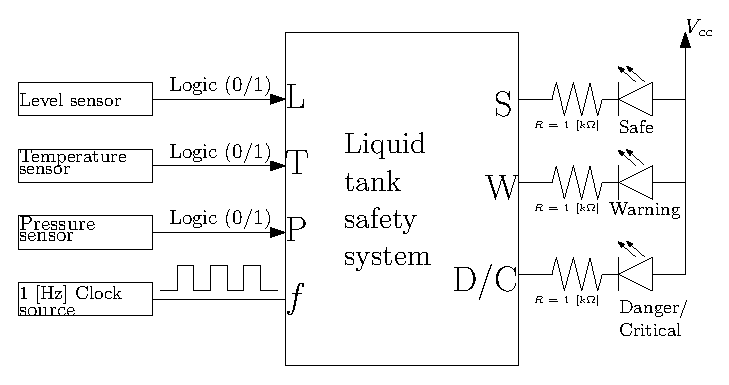
\includegraphics{figs/ipe/lab_10/safetySys.eps}
    \caption{Block diagram of the chemical tank safety system using active-low logic.}
    \label{fig:safetySys}
\end{figure}
%
The behavior of the liquid tank safety system is different than that of the safety system designed with the active-high logic in the previous section. The tank is safe only when no sensor is active (\textit{i.e.,} none of the sensors indicate that the tank's measuring quantity: liquid, temperature, or pressure exceeds their threshold values). The warning, danger, and critical LEDs  illuminate  when one, two, and all three sensors generate active-high signals. The danger and critical signals use the same (red) LED. The safety system in this case has a clock source $f$ ($f=1$~[\hertz]) as an additional input to the safety system. The anode terminals of the LEDs are now connected to a voltage source $V_{\text{cc}}.$  
%
%
Table~\ref{tab:truthTableTank2} shows the input combinations (sensors) for which  the  safe ($S$) and the warning ($W$) signals are active-low (\textit{i.e.,} green and yellow LEDs are ON). %
%
\begin{table}  
  \centering
  \caption{Truth (function) table of the liquid tank safety system (safe and warning) shown in Figure~\ref{fig:safetySys} (block diagram).}  
  \begin{tabular}{ccc|c|c}
    \toprule
    L & T & P & S & W\\
    \toprule
    0 & 0 & 0 & 0 & 1\\
    0 & 0 & 1 & 1 & 0\\
    0 & 1 & 0 & 1 & 0\\
    0 & 1 & 1 & 1 & 1\\
    1 & 0 & 0 & 1 & 0\\
    1 & 0 & 1 & 1 & 1\\
    1 & 1 & 0 & 1 & 1\\
    1 & 1 & 1 & 1 & 1\\
    \bottomrule
  \end{tabular}
  \label{tab:truthTableTank2}
\end{table}
%
The Boolean expressions for the safe $(S)$ and warning $(W)$ signals are: %
%
\begin{subequations}
\begin{align}
  \label{eq:S-AL}
  S(L,T,P) &= (L^{'}T^{'}P^{'})^{'} = L+T+P\\
    \label{eq:W-AL}
  W(L,T,P) &= (L^{'}T^{'}P + L^{'}TP^{'}+LT^{'}P^{'})^{'}
\end{align}  
\end{subequations}
%
However, the danger/critical LED has three states: ON, OFF, and flashing. Therefore, the state of the danger/critical LED relies on  the clock source (additional input) and its status is described by the truth table shown in Table~\ref{tab:truthTableTank3}. Note that the D/C output  employs the active-low logic. Therefore, the danger/critical  LED is ON (OFF) when the  D/C output  is $0~(1).$

When two sensors are ON, the D/C LED is ON regardless of the state of the clock source $f.$ However, the D/C LED should be flashing when all three sensors are ON. The input combinations $STPf = 1110$ and $STPf = 1111$ will make the D/C LED ON and OFF (flashing), respectively. %
%
\begin{table}  
  \centering
  \caption{Truth (function) table  of the liquid tank safety system (danger/critical) shown in Figure~\ref{fig:safetySys} (block diagram).}  
  \begin{tabular}{cccc|c}
    \toprule
    L & T & P & f & D/C\\
    \toprule
    0 & 0 & 0 & 0 & 1\\
    0 & 0 & 0 & 1 & 1\\
    0 & 0 & 1 & 0 & 1\\
    0 & 0 & 1 & 1 & 1\\
    0 & 1 & 0 & 0 & 1\\
    0 & 1 & 0 & 1 & 1\\
    0 & 1 & 1 & 0 & 0\\
    0 & 1 & 1 & 1 & 0\\
    1 & 0 & 0 & 0 & 1\\
    1 & 0 & 0 & 1 & 1\\
    1 & 0 & 1 & 0 & 0\\
    1 & 0 & 1 & 1 & 0\\
    1 & 1 & 0 & 0 & 0\\
    1 & 1 & 0 & 1 & 0\\
    1 & 1 & 1 & 0 & 0\\
    1 & 1 & 1 & 1 & 1\\    
    \bottomrule
  \end{tabular}
  \label{tab:truthTableTank3}
\end{table}
%
The Boolean expression for the D/C output is given as: %
%
\begin{align}
  D/C(L,T,P) = (L^{'}TP + LT^{'}P + LTP^{'} + LTPf^{'})^{'}
  \label{eq:dangerCritical-AL}
\end{align}
%
The Boolean expression for the danger/critical output given in~\eqref{eq:dangerCritical-AL} can be implemented with one 4-input AND gate, three 3-input AND gates, one 4-input OR gate, and five NOT gates (\textit{i.e.~} inverters).  

\section{Prelab}
\label{sec:prelab}
Before you start working on the prelab, it is important to read the problem description given in section~\ref{sec:introduction}.  The prelab consists of two parts that cover the preliminary analysis of the combinational logic circuit that implements a simple liquid tank (sealed) safety system.
%
% It consists of two parts. In the first part, the safety system is implemented with active-high logic. In the second part, active-low logic is utilized to implement the liquid tank safety system. %
%
\begin{prelab}[Liquid tank safety system (active-high logic)]{prelab:tankSafetySystemActiveHigh}
  Consider the safety system given by the block diagram shown in Figure~\ref{fig:safetySysNoClock}.
  
  \begin{enumerate}
    \item From Table~\ref{tab:truthTableTank1}  write the logic expressions for the three output (Boolean) variables $S,$ $W,$ and $D$ in terms of inputs.
  % 
  \begin{align*}
    &S(L,T,P) = \ldots \\
    &W(L,T,P) = \ldots \\
    &D(L,T,P) = \ldots \\    
  \end{align*}
  %

\item Simplify the logic expressions for the output variables found in the previous step. %
\item  Draw the logic circuit diagram of the liquid tank safety system shown in Figure~\ref{fig:safetySysNoClock}.
\end{enumerate}
\end{prelab}

\begin{prelab}[Liquid tank safety system (active-low logic)]{prelab:tankSafetySystemActiveLow}
Consider the safety system given by the block diagram shown in Figure~\ref{fig:safetySys}. 
%
\begin{itemize}  
\item  Draw the logic circuit diagram of the liquid tank safety system shown in Figure~\ref{fig:safetySys}.
\end{itemize}
\end{prelab}

\section{Laboratory Work}
To conduct this experiment, the Agilent E3630 $\mathbf{0}$-$\mathbf{6}~[\volt]$ power supply (already available at the workstation) is needed for the logic gate ICs to supply  $V_{\mathrm{cc}} = 5~[\volt].$ 

\begin{mdframed}
  {\bf NOTE: HAVE YOUR INSTRUCTOR OR A TEACHING ASSISTANT CHECK YOUR LOGIC CIRCUIT BEFORE TURNING IT ON.}  
\end{mdframed}


\subsection{Part~1: Tank Safety System using Active-High Logic}
\label{sec:part1}


\begin{enumerate}
\item Check each gate of the AND, OR, and NOT gate ICs using two inputs and one output connected to an LED (a $1~[\kilo\ohm]$ resistor must be connected in series with the LED).
  
\item Build the logic circuit for the expressions of the outputs $S(L,T,P),$ $W(L,T,P),$ and $D(L,T,P)$ (see logic expressions you derived  in Prelab \#1).
  
\item Check your circuit with different combinations of inputs and complete the following table for the outputs:

  \begin{center}
  \begin{tabular}{ccc|c|c|c}
    \toprule
    L & T & P & S & W & D\\
    \toprule
    0 & 0 & 0 & $\ldots$ & $\ldots$ &  $\ldots$\\
    0 & 0 & 1 & $\ldots$ & $\ldots$ &  $\ldots$\\ 
    0 & 1 & 0 & $\ldots$ & $\ldots$ &  $\ldots$\\ 
    0 & 1 & 1 & $\ldots$ & $\ldots$ &  $\ldots$\\ 
    1 & 0 & 0 & $\ldots$ & $\ldots$ &  $\ldots$\\ 
    1 & 0 & 1 & $\ldots$ & $\ldots$ &  $\ldots$\\ 
    1 & 1 & 0 & $\ldots$ & $\ldots$ &  $\ldots$\\ 
    1 & 1 & 1 & $\ldots$ & $\ldots$ &  $\ldots$\\ 
    \bottomrule
  \end{tabular}
\end{center}

\item Comment on any discrepancy found between the Truth table  outputs shown in Table~\ref{tab:truthTableTank1} and the experimental outputs found in the previous step. 
\end{enumerate}


\subsection{Part~2: Tank Safety System using Active-Low Logic}
\label{sec:part2}
\begin{enumerate}
\item Build the logic circuit for the expressions of the outputs $S(L,T,P)$ and $W(L,T,P)$ given in Equations~\eqref{eq:S-AL} and \eqref{eq:W-AL}, respectively. 
  
\item Test your circuit with different combinations of inputs and check the outputs with the truth table shown in Table~\ref{tab:truthTableTank2}.

\item Build the logic circuit for the expression of the output $D/C(L,T,P)$ given in Equation~\eqref{eq:dangerCritical-AL} and check its operation (\textit{i.e.,~} output) with  the truth table shown in Table~\ref{tab:truthTableTank3}. [Use  the function generator \textbf{sync output} to provide $1~[\hertz]$ pulse to the $f$ input].

\item Comment on any discrepancy found between the Truth table  outputs shown in Tables~\ref{tab:truthTableTank2}~and~\ref{tab:truthTableTank3}, and the experimental outputs found in the previous steps. 
\end{enumerate}

% \section{Deliverables}
% Record all your measurements and analysis in your lab notebook and submit the notebook in the next lab session. 
%Good luck on your Finals and have a relaxing Christmas Break!

% \begin{itemize}
% \item Demonstrate your work to the Professor or the GA before leaving the lab. 
% % \item Upload labDC\_Motor2\_Main.vhdl through Sakai under \emph{Assignments/labDC-Motor2-Main (FPGA--based motor control)}
% \item No report (or notebook)  is required for this lab.
% \end{itemize}

% \begin{thebibliography}{9}
% \bibitem{Buchla2010} 
% David M. Buchla.
% \textit{Experiments in Electronics Fundamentals and Electric Circuits Fundamentals}. 
% Pearson Education, Inc., 2010.

% \end{thebibliography}



%%% Local Variables:
%%% mode: latex
%%% TeX-master: "../../labHandoutECE227-V1"
%%% End:
